\section{Uma Primeira Seção para o Apêndice}

A matriz de Dilema Linear $M$ e o vetor de torques inerciais $b$,
utilizados na simulação são calculados segundo a formulação 
abaixo:
\begin{equation}
M=\left[ \begin{array}{ccc}
M_{11} & M_{12} & M_{13} \\
M_{21} & M_{22} & M_{23} \\
M_{31} & M_{32} & M_{33}
\end{array} \right]
\end{equation}

\begin{figure}[h]
\centering
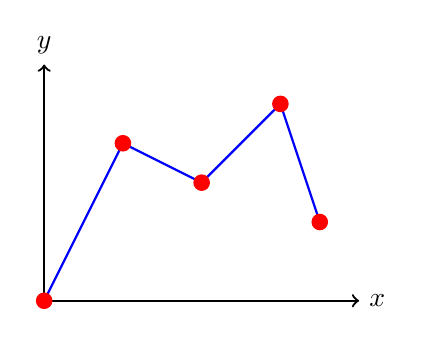
\begin{tikzpicture}
  \draw[thick, ->] (0,0) -- (4,0) node[right] {$x$};
  \draw[thick, ->] (0,0) -- (0,3) node[above] {$y$};
  \draw[blue, thick] (0,0) -- (1,2) -- (2,1.5) -- (3,2.5) -- (3.5,1);
  \foreach \x/\y in {0/0, 1/2, 2/1.5, 3/2.5, 3.5/1} {
    \fill[red] (\x,\y) circle (3pt);
  }
\end{tikzpicture}
\caption{Exemplo de figura em apêndice.}\label{FD}
\end{figure}
